\documentclass[a4paper,12pt]{article}

\usepackage{tikz}
\usetikzlibrary{decorations.pathreplacing}
\usepackage{amsmath}
\usepackage{amsfonts}
\usepackage{amssymb}
\usepackage[margin=1in]{geometry}
\usepackage{graphicx}
\usepackage[]{geometry}
\usepackage{inconsolata}
\usepackage{courier}
\usepackage{listings}
\usepackage{enumerate}
\usepackage{float}
\usepackage{answers}
\usepackage[english]{babel}
\usepackage{commath}
\usepackage[labelfont=bf]{caption}
\usepackage{mwe}
\usepackage[longnamesfirst]{natbib}
\usepackage{algorithm}
\usepackage[noend]{algpseudocode}
\usepackage{eurosym}
\usepackage{siunitx}
\usepackage{ctable}
\usepackage{subfig}
\usepackage{dsfont}

\setlength{\parindent}{0pt}
\setlength{\parskip}{1em}

\title{Maintenance Policies for a Multi-Unit System with Adjustable Production Rates}
\author{Mark van der Broek}
\date{\today}

\begin{document}
	
	\maketitle

\section{Introduction}	
% Good maintenance policies are required
Maintenance cost can constitute a large part of the total production costs. For example, \cite{GRABER2004861} states that maintenance costs can be at much as 30 percent of production costs for power plants, while \cite{BEVILACQUA200071} give an estimate of between 15 and 70 percent of the total production costs. For this reason, maintenance strategies have been extensively researched in the past decades. Reviews of past research have been published (CITE). Condition-based maintenance (CBM) is an advanced maintenance strategy that is based on performance and/or parameter monitoring and basing subsequent actions on the monitoring. 

Condition-based maintenance policies have been proposed for multi-unit systems with economic dependence \citep{OLDEKEIZER2016531}. \cite{OLDEKEIZER2018319} extend this research by including load sharing between units, that is, the deterioration of the functioning units is affected by the number of functioning units, where it is assumed that the load is shared uniformly over all functioning units. In this paper we consider a system where we relax this assumption and allow the load of all functioning units to depend on the current deterioration level of these units.

The coupling of production and maintenance has been the subject of several studies in recent years. Li and Ni (2009 Jin, X., L. Li, and J. Ni. 2009. “Option Model for Joint Production and Preventive Maintenance System.” International Journal of Production Economics 119(2): 347–353.
[Crossref], [Web of Science ®], [Google Scholar]
) present an option-based cost model for scheduling a joint production and maintenance policy for a single-period, single-product system.


Offshore wind farms is one of the renewable energy solutions. Since the operation and maintenance costs represent a substantial portion of the total life cycle costs of these offshore wind farms \cite{hau2003wind}, reliability and condition strategies have drawn increasing interest for decreasing these costs, e.g. \cite{krokoszinski2003efficiency}. Existing CBM methods for offshore wind farm systems deal with wind turbines as individual components separately \citep{avner2007reliability}. Later maintenance strategies where economic dependence for maintenance actions between wind turbines is taken into account have gained interest \citep{tian2011condition}. The authors claim a maintenance costs reduction of up to 44.42\% compared to maintenance strategies that do not take the economic dependence into account. This reduction is mostly due to the fact that it exploits the large fixed costs from and cluster maintenance actions. One element of the fixed costs component is the cost of sending a maintenance team to the wind farm,, which generally requires expensive vessels.

In this paper, we consider a joint production and maintenance strategy for a multi-unit system. We formulate the system as a Markov Decision Process and analyse the structural properties of the optimal policies. Our model extends the model of \cite{OLDEKEIZER2018319} by allowing the load sharing to be set for all units. The deterioration process of the units is modelled by a discrete-time Markov chain with a known transition probability matrix. The load sharing and maintenance strategy are jointly optimised, while in traditional methods the load sharing is set be uniform for all units. 

The remainder of the paper is organised as follows. Section 2 provides the definition and formulation of the system. Section 3 provides a description of the Markov Decision Process used to model the system introduced in Section 2. In Section 4 and 5 the structural properties of the optimal policies of a system with respectively 2 and 3 units is analysed. Conclusions and future research directions are provided in Section 6.
% For systems with multiple units, there exists dependence between the units. 

% Windmills require expensive fixed costs, so clustering maintenance can be profitable. In many windmill contracts a specified production has to be met for the total windpark. Try to combine production with maintenance policies.


\section{System formulation}
We consider a discrete-time system consisting of $N$ identical components, which are subject to load sharing and economic dependence. We denote the set of units as $\mathcal{I} = \{1, \dots, n\}$. The total load that has to be met during every time period is denoted $\pi$.  Let $x_i$ denote the deterioration state of unit $i$, which deteriorates according to a discrete-time Markov chain with deterioration states $X = \{0, 1, \dots, L\}$. State $0$ represents the as-good-as-new state, $L-1$ denotes the most deteriorated state such that the unit still functions and state $L$ the failed state. We assume that the load capacity of a unit is not affected by the deterioration state. A schematic overview of the events in one time period is presented in Figure 1.

\begin{figure}[H]
	\centering
	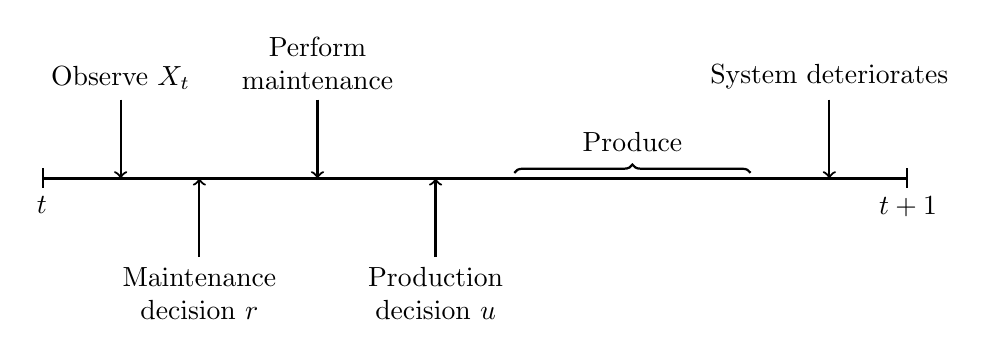
\begin{tikzpicture}
	\coordinate (t) at (0,0);
	\coordinate (X) at (1,0);
	\coordinate (R) at (2,0);
	\coordinate (M) at (3.5,0);
	\coordinate (U) at (5,0);
	\coordinate (UE) at (9,0);
	\coordinate (D) at (10,0);
	\coordinate (t+1) at (11,0);
	
	% Draw the time horizon
	\draw[thick, |-|] (t) -- (t+1);
	\draw (t) node[below=3pt] {$t$};
	\draw[thick, ->] (1,1) node[above, align=center] {Observe $X_t$} -- (X);
	\draw[thick, ->] (2,-1) node[below, align=center] {Maintenance \\ decision $r$} -- (R);
	\draw[thick, ->] (3.5, 1) node[above, align=center] {Perform \\ maintenance} -- (M);
	\draw[thick, ->] (5, -1) node[below, align=center] {Production \\ decision $u$} -- (U);
	\draw[thick, decorate, decoration={brace,raise=2pt, amplitude=3pt}] (6,0) -- (9, 0) node[sloped,midway, above=6pt] {Produce};
	\draw[thick, ->] (10, 1) node[above, align=center] {System deteriorates} -- (D);
	\draw (t+1) node[below=3pt] {$t+1$};
	\end{tikzpicture}
	\caption{Order of events for time epoch $t$.}
\end{figure}

\subsection{Maintenance and load actions}
The deterioration state of each unit is known at the beginning of each time period. This assumption becomes is justified for an increasing number of applications, due to better monitoring equipment. Maintenance is assumed to take negligible time and is performed after the deterioration states of each unit is observed. Preventive maintenance is performed at a cost of $c_\text{pm}$ if the unit has not reached the failed state, whereas a corrective maintenance action is performed in the failed state at a cost of $c_\text{cm}$. Generally, the cost of preventive maintenance is lower than the corrective maintenance action ($c_\text{pm} < c_\text{cm}$). Performing maintenance on a unit instantanously brings it back to the as-good-as new state. The economic dependence is included in the form of a fixed cost $C$ for performing maintenance for a time period. The cost is incurred when at least one unit will be maintained.

After selecting the maintenance action, we also have to set the production rate of each unit. Each unit can produce at most $m+1$ different production rates, ranging from $0$ to $1$ (maximum production). The possible production rates are uniformly distributed over the interval. If a unit is in the failed state, we cannot produce, so the production rate of this unit is set to $0$. For all other deteriorating levels, we can select one of the $m+1$ production rates.


\subsection{Deterioration Process}
Each unit $i$ deteriorates according to a gamma process with rate $\lambda(u_i)$, which depends on the current production rate of the unit, and scale parameter $\gamma$. The rate for a given production rate $u_i$ is given by
$$
\lambda(u_i) = g(u_i) \lambda_{\text{max}},
$$
where $\lambda_{\text{max}}$ is the rate parameter under the maximum production rate, and $g$ is a non-decreasing function. We assume that $g(u_i)$ as a function of the production rate $u_i$ for unit $i$ is of the following form
$$
g(u_i) = \beta + (1-\beta)u_i^\alpha.
$$
We assume that $0 \leq \beta \leq 1$ and $\alpha \geq 0$, since $g$ should be non-decreasing in $u_i$. If the production rate $u_i$ is zero, then $g$ has value $\beta$ i.e., $\beta$ determines the deterioration rate if the unit does not produce.  The parameter $\alpha$ determines the curvature of the function $g$. In Figure 2 the function $g$ is plotted for several settings of $\alpha$ and $\beta$. 

\begin{figure}[H]
	\centering
	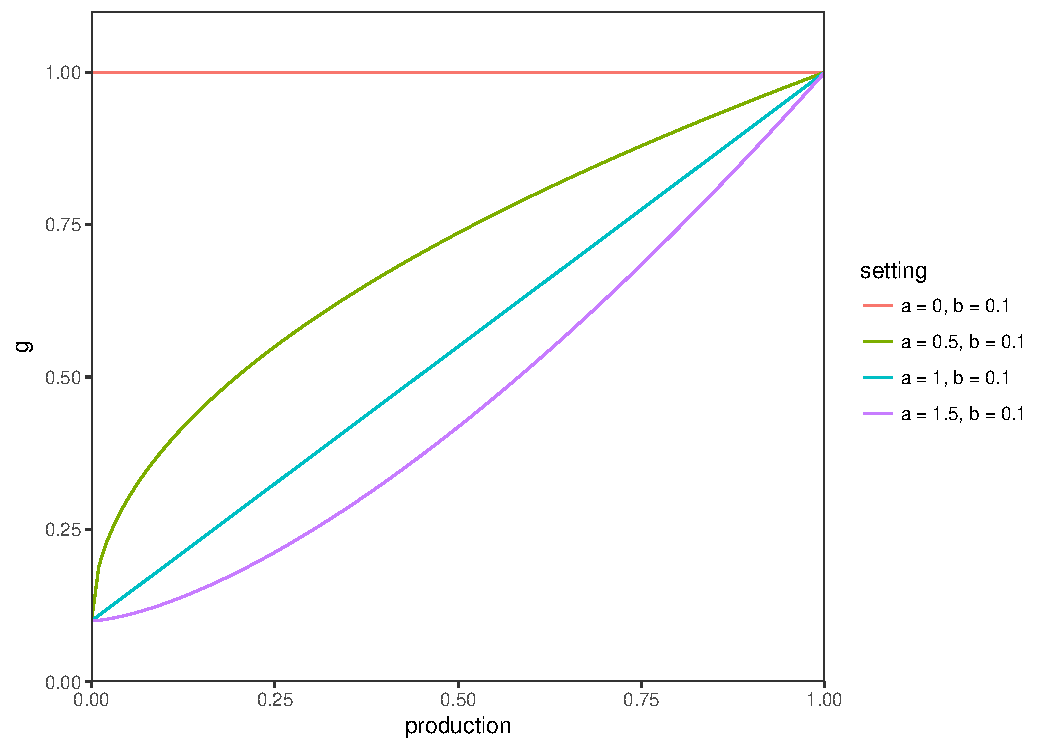
\includegraphics[width=0.5\linewidth]{figures/g}
	\caption{Function $g$ for values $\alpha = 0, 0.5, 1, 1.5$ and $\beta = 0.1$.}
\end{figure}

The discrete jump probabilities for the gamma process are obtained by discretising the gamma process. One property of the gamma process is that the jump probabilities are independent of the current state. We denote the probability of having a jump of size $j$ with rate parameter $a$ and scale parameter $b$ by $p(i; a, b)$. The derivation of the jump probabilities can be found in the manuscript by De Jonge on pages 51-53.

\section{Markov Decision Process}
In this section I provide the Markov Decision Process (MDP) formulation of the system as described in Section 2. The MDP consists of a state space, action space, transition probabilities, expected costs and a performance evaluation.

\subsection{State space}
We consider a multi-unit system that consists of $n$ identical units. We denote the set of units as $\mathcal{I} = \{1, \dots, n\}$. Each unit deteriorates according to a discrete-time Markov chain with deterioration states $X = \{0, 1, \dots, L\}$. State $0$ represents the as-good-as-new state and state $L$ the failed state. The whole state of all units is denoted by
$$
x = (x_1, \dots, x_n) \in X^n.
$$

\subsection{Action space}
At the start of each time unit we have to decide on which components to maintain (M) and do nothing (DN). Maintenance can be performed one all units, independent of the current state, i.e., the action space for the maintenance decision can be defined as
$$
R = \left \{r = (r_1, \dots, r_n): r_i \in \{\text{DN}, \text{M}\}, \enskip \forall i \in \mathcal{I} \right \}.
$$

 We define the set of possible production rates for unit $i$ in state $x_i$ $U(x_i)$ as follows
$$
U(x_i) = \begin{cases}
\{0, 1/m, \dots, 1\} & \text{ if } x_i \neq L, \\
\{0\} & \text{ if } x_i = L.
\end{cases}
$$
Let $u = (u_1, \dots, u_n)$ denote the production rate of all units in the system. The total production of the system is restricted to $\pi$, i.e., $ \sum_{i=1}^{n}u_i = \pi$. This results in the following action space for the system in state $x$
$$
U(x) = \left\{ u  :  \sum_{i=1}^{n}u_i = \pi, u_i \in U(x_i) \enskip \forall i \in \mathcal{I} \right\}.
$$
Note that the production action space decreases from $(m+1)^n$ elements to ${n + \pi - 1} \choose{\pi - 1} $ by restriction the total production rate to the value $\pi$. 

\subsection{Transition probabilities}
For a unit $i$ the probability of having $q \geq 0$ jumps in the deterioration states for a time epoch under production rate $u_i$ and scale parameter $b$ is given by $p(q; \lambda(u_i), b)$. The transition probability of unit $k$ for going from state $i$ to $j$ with production rate $u_i$ and maintenance action DN for any time epoch is defined as
$$
P_{u_k,\text{DN}}(i,j) = \begin{cases}
p(j-i; \lambda(u_k), b) &\text{ if } i \leq j \leq L-1, \\
0 &\text{ if } j < i, \\
1 - \sum_{l=0}^{L-1-i}p(l; \lambda(u_k), b) & \text{ if } i \leq m-1  \text{ and } j = L, \\
1 & \text{ if } i = j = L,
\end{cases}
$$
and for maintenance action M by
$$
P_{u_k,\text{M}}(i,j) = \begin{cases}
p(j; \lambda(u_k), b)&\text{ if } j \leq  L-1, \\
1 - \sum_{l=0}^{L-1}p(l; \lambda(u_k), b) & \text{ if } j = L.
\end{cases}
$$
Note that for the maintenance action M the probability of going from state $i$ to $j$ does not depend on $i$, since we assume that the system will go to state 0 immediately after the maintenance action.

The transition probability of a unit in the system is independent of the other units. Therefore, the transition probability that the system goes from state $x = (x_1, \dots, x_n)$ to state $\tilde{x} = (\tilde{x}_1, \dots, \tilde{x}_n)$ by selecting production rates $u$ and maintenance actions $m$ is given by
$$
p(x, \tilde{x} \mid u, m) = \prod_{i = 1}^nP_{u_i,m_i}(x_i, \tilde{x}_i),
$$
due to independence of the deterioration process of the units.



\subsection{Expected costs}
To define the cost for a time unit, we define a function
$$
c(x_i,r_i) = \begin{cases}
c_{\text{pm}} & \text{ if } r_i = \text{M} \text{ and } x_i \neq L, \\
c_{\text{cm}} & \text{ if } r_i = \text{M} \text{ and } x_i = L, \\
0 & \text{ elsewhere}.
\end{cases}
$$
for all states $x_i \in X$ and maintenance actions $r_i \in \{\text{DN}, \text{M}\}$ of unit $i \in \mathcal{I}$. This means that if unit $i$ is in the failed state and we decide to perform maintenance, we incur the corrective maintenance costs $c_{\text{cm}}$, and if the unit has not failed, then the preventive maintenance costs $c_{\text{pm}}$ is incurred. 

The expected costs for a time unit by selecting maintenance action $r$ and in state $x$ is given by
$$
\bar{c}(x,r) = \begin{cases}
C + \sum_{i=1}^{n}c(x_i, r_i), &\text{if } r \text{ contains a maintenance action},\\
0, &\text{otherwise}.
\end{cases}
$$
In words, this means that if we do not perform maintenance on any unit for a given time period, we do not incur any costs. However, if we do perform maintenance, we incur the fixed cost $C$ and some corrective or preventive costs depending on the state of the maintained unit.
\subsection{Performance criteria}
As a performance criterion, we are interested in minimising the long-run average cost per time unit. In this way we can quantify the maintenance costs of a system over the life cycle, and identify the benefits of being able to set the load of each unit. 

\section{Numerical results two-unit system}
In this Section we will investigate the key features of the optimal maintenance and production policy for a two-unit system using the MDP as described in Section 3. Similar to \cite{OLDEKEIZER2018319} we select preventive maintenance costs $c_\text{pm} = 5$, set-up cost $C = 4$, and a corrective maintenance cost $c_\text{cm} = 11$. The rate parameter under the maximum load rate is $\lambda_{\text{max}} = 0.7$ and the scale parameter $\gamma = 1$. The failure level $L$ and the number of possible production rates are set to 30. We vary the total load $\pi$ with values 30, 40 and 50. For $\pi = 50$, one unit can handle all the load and for $\pi = 50$ we do not have much overcapacity in the system. We set $\alpha = 0.1$, such that the deterioration when a unit is not operating is low. We consider three different values for $\beta$:  $0$ (deterioration rate does not depend on production), $1$ (deterioration rate depends linearly on production) and $1.5$ (deterioration rate is convex in the production).




\subsection{Benchmark policies}
Since the action space of our problem consists of a maintenance action and a production action, we distinguish between a benchmark for the maintenance action and the production action. 

In the literature, condition-based maintenance is often implemented in the form of a threshold policy (CITE), or an opportunistic threshold policy \citep{ZHANG2015176}. In the former policy, if the deterioration level of a unit is at or exceed a threshold level $T_r$, we perform a maintenance action. The opportunistic policy adds an additional step to the threshold policy: if an maintenance action is initiated, then all units that have a deterioration state higher or equal to $T_o$ are also maintained in that time period. The optimal threshold values for $T_r$ and $T_o$ are found using a grid search procedure. Due to the economic dependence (fixed cost of maintenance) and the liberty to set the production rate of the components, this policy is probably not optimal.

\textbf{[[Note: I think it is unfair to compare the optimal policy to the standard threshold policy, since this policy is equal or worse than the opportunistic policy. ]]}

Additionally, we need a benchmark policy for the production policy. Inspired by the load sharing formulation in \cite{OLDEKEIZER2018319}, we will use the following benchmark for the production policy: For all system states determine the optimal selection of functioning units, where all functioning units share the load uniformly. The optimal selection is found by minimising the long-run average  cost per time unit.

Table (???) presents the 



\subsection{Sensitivity analysis}
\begin{enumerate}
	\item Effect of fixed costs. More or less clustered maintenance.
	\item Effect of variance.
	
\end{enumerate}

\section{Numerical results three-unit system}

\section{Conclusion}
% Summary

% Future research
In this paper, I do not include dependence between the capacity of units and its deterioration state. 

\bibliographystyle{IEEEtranSN} 
\bibliography{mylib}

\appendix

\section{Appendix}

\subsection{Discretising the gamma process}
See Maintenance planning and optimisation literature of Bram de Jonge.

\end{document}


